%-----------------------------------------------------------------------------------------------------------
\chapter{INTRODUCTION} % Main chapter title
\label{Introduction} % For referencing the chapter elsewhere, use \ref{Chapter1} 
\lhead{Chapter 1. \emph{Introduction}} % The header on each page
%-----------------------------------------------------------------------------------------------------------

\section{Historical Background}
\hspace{30}Throughout our long history, we humans have always sought for means 
to express our creativity–ways to communicate our ideas through writing, 
sculpting, painting, carving, architecture and drawing.As a matter of fact,
paleolithic cave representations of animals at least 32,000 years ago in  
Southern France, ink drawings and paintings of human figures as well as writings 
in hieroglyphics on papyrus in the pyramids of ancient Egypt is
indicative of the fact that our need to express our individuality goes back to
antiquity.Before the renaissance, drawing was treated as a preparatory stage
for painting and sculpting.The wide availability of drawing instruments such as 
pens and pencils and most especially paper made master draftsmen like
Leonardo Da Vinci, Raphael and Michelangelo around the world to lift drawing
to an art in its own right.Thus, drawing stood out as the most popular and
fundamental means of public expression in human history and is one of the
simplest and most efficient means of communicating visual ideas.\cite{1}\\

\hspace{30}The drawing board era where paper, pens, pencils, rulers and ink  
prevailed has been relegated to the background in this information age which is  
powered by ubiquitous computer technology. Craving the unity of science and  
art, this essentially binary­-sequenced revolutionary device called the computer  
married the artistic and engineering forms of drawing into an androgynous one  
called Computer­Aided Geometric Design or geometric modeling for short.
Geometric modeling currently involves the use of computers to aid in the  
creation, manipulation, maintenance and analysis of representations of the  
geometric shapes of two and three­dimensional objects \cite{2}. It is the outgrowth  
of convergent motivations and developments from several works of life as  
outlined below.
\begin{itemize}
\item In the 1950s, the need to automate the engineering drawing process led
to electronic drawings which could be archived and modified more easily,
could be easily verified and errors could be eliminated from mechanical 
designs without introducing new ones.These computer drafting systems
allowed designers to produce drawings of objects by projecting
three­dimensional objects unto two­dimensional surfaces.
\item Then in the 1960s, there was a pressing need for software in the
automobile, shipbuilding and aircraft industries to produce
computer-­compatible descriptions of geometric shapes which can be
machined from wood and steel into stamps and dies for the
manufacturing and assembling of car parts,ship hulls as well as wings and  
fuselages using computer numerically controlled tools.
\item Later in the 1970s, the growing need for computers to render realistic
images of objects as well as animate solid objects pushed research
institutes like Xerox Palo Alto Research Center (Xerox PARC) and Apple
Computers to make significant contributions to graphical user­ interface
design and computer graphics.  
\end{itemize}

These needs and problems could only be solved by research in fields such as
graphics, animation and applications from algebraic geometry. The work of
various computer scientists and mathematicians lead to the active development
of several commercial packages sponsored by companies such as Renault,
Citroen, Ford and Boeing who could afford the computers capable of  
performing such lengthy calculations.  

\hspace{30} Today,geometric modeling is also referred to as Computer ­Aided Design
(CAD), is pronounced “cad” and is routinely used in the design and
manufacturing of engineering and architectural structures such as buildings, car  
parts, ship hulls and aircraft artillery as well as to specify special effects in  
cartoon movies, music videos and television shows. Indeed, CAD packages
provide facilities for designing shapes of solid physical objects and specifying
their motion in a way that art and science can unite to create cool designs.  

\hspace{30} Even though significant progress had been made in basic research and
the functionality of commercially available solid modelers like Apple
Computer's RenderMan, many solid modelers especially within the open
source community are still limited in their geometric features. The open
source community is a self­organizing collaborative social network of 
programmers driven by a passion to solve problems using computers.
It has several thousands of its projects on sites that offer services 
like bug tracking, mailing lists and version control viz \href{https://github.com/}{Github} 
and \href{http://sourceforge.net}{Source Forge}.These projects are constantly 
being improved upon by thousands of programmers putting in time and effort 
to write and debug software without direct monetary pay.

\hspace{30} In this thesis, we document the process of developing a heart­-shaped
primitive, a set of callback functions and procedures which compute geometrically 
useful properties of solids such as wireframe plotting, database importation and 
exportation,ray tracing, bounding box calculations, just to name a few, within the
 Ballistic Research Laboratory Computer Aided Design (BRL-­CAD) software package.  

\hspace{30} BRL-­CAD was initiated by the United States Army Research Laboratory
in 1983, the same agency which created the E.N.I.A.C., the world's first 
general ­purpose computer in the 1940s, to model military systems for the
United States government. According to \cite{3}, BRL-­CAD became born again in 
2004 when it joined the open source community with portions of its source
code licensed under the Lesser General Public License (LGPL) and Berkeley
Software Distributions (BSD) licenses and has been credited as being the
oldest open source repository in continuous development. It supports a wide
variety of geometric representations including an extensive set of traditional
implicit primitive shapes as well as explicit primitives made from collections of
uniform B­spline surfaces, Non­uniform Rational B­spline (NURBS) surfaces,  
Non­manifold geometry (NMG) and purely faceted polygonal mesh geometry.  

\hspace{30} BRL­-CAD also focuses on solid modeling aspects of Computer ­Aided
Design. Figure 1.1 below shows a three­dimensional model of a Goliath tracked
mine, a German engineered remote controlled vehicle used during World War II.
This model was created by students new to BRL-­CAD in the span of about 2
weeks, starting from actual measurements in a museum.

%----------------------------------------------------------------------------------------

\section{Importance Of This Work}

This work is significant to several stakeholders for several reasons ;

\begin{itemize}
\item By ray­tracing the heart's surface, it demonstrates to the scientific
community that the Laguerre zero­finder is indeed a sure­fire iterative
method for finding roots of polynomials and that Laguerre-­based root 
solvers are stable on sextic equations.
\item This work incorporates more geometric modeling functionality into 
the free and open source software community through BRL-­CAD, the oldest open 
source repository in continuous development\cite{3} by going beyond traditional 
CSG primitives shapes such as tori, spheres, boxes and ellipsoids towards the more
complex heart-shape based on a sextic equation. This work provides a guideline 
for the development of primitives within open source CAD software.
\item Given that BRL­-CAD is used within governments to model military artillery
 and for engineering and analysis purposes within academia, this
heart­-shaped primitive gives BRL-­CAD a more loving aura – an 
environment where artists can produce cartoon animations as well as
design cards, royal seals and banners, gifts and presents for family and
communal celebrations such as weddings, family reunions and
Valentine's day for entertainment purposes.
\end{itemize}

%--------------------------------------------------------------------------------------------

\section{Thesis Organisation}

This thesis is divided into five (5) chapters. Chapter 1 introduces the study and chapter 2 reviews the literature in the field of geometric modeling. In Chapter 3, we state the problems we intend to solve and our project design. In chapter 4, we discuss the interesting results which we obtained. Finally, in
chapter 5, we state the contribution of our work and give possible research
directions which can proceed from it.

%--------------------------------------------------------------------------------------------

\begin{figure}[htbp]
\centering
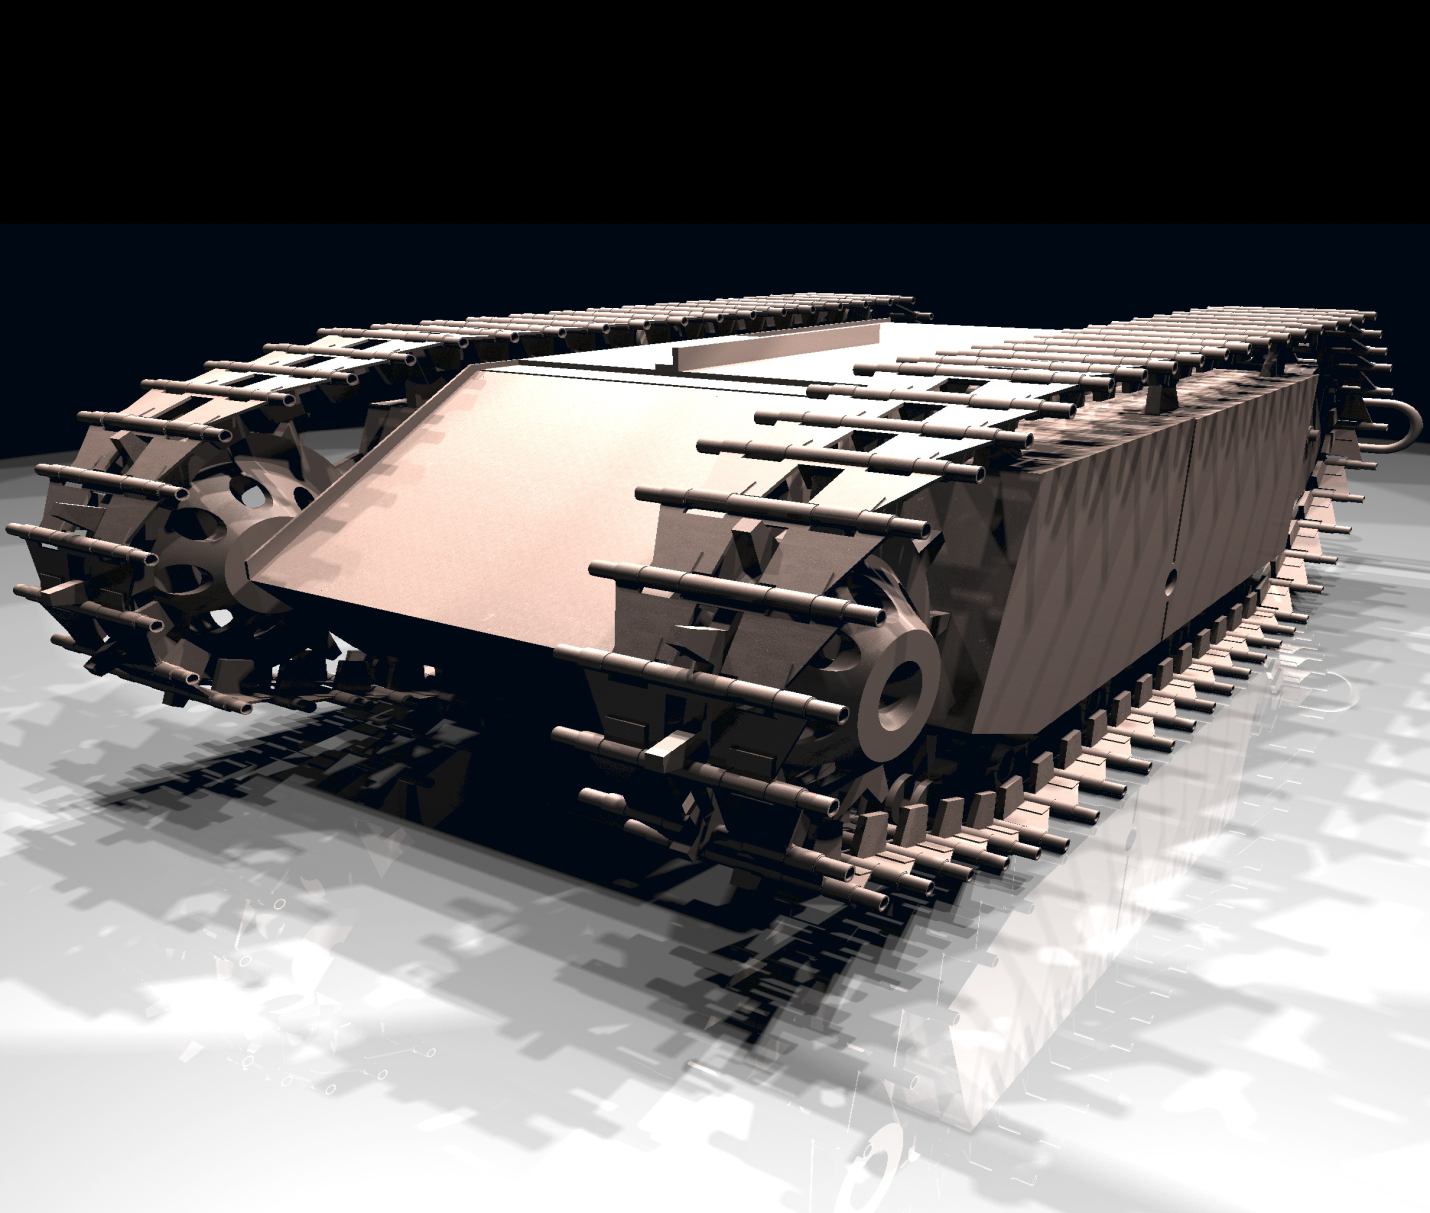
\includegraphics[trim=1cm 2cm 3cm 4cm, clip=true, totalheight=0.5\textheight]{Figures/Goliath.png}
\caption[Model of a Goliath tracked mine]{Model of a Goliath tracked mine}
\label{Goliath}
\end{figure}

%--------------------------------------------------------------------------------------------
